\documentclass{article}
\usepackage[utf8]{inputenc}

\usepackage[letterpaper, margin=1in]{geometry}
\usepackage{amsmath}
\usepackage{enumitem}
\usepackage{caption}
\usepackage{subcaption}
\usepackage{graphicx}
\graphicspath{ {figures/} }

\title{Analytical model of pedestrianized and transit priority zones in a rectilinear grid city}
\author{Nicholas Fournier and Eric Gonzales}
\date{February 2020}

\begin{document}


\maketitle

\section{Concept}
Consider an idealized city of dimension $R$ with a rectilinear street network with spacing $d$, as shown in Figure~\ref{fig:gridcity}. Demand can be defined by two types of trip patterns, baseline uniform travel demand across the city and monocentric trips to and from the city center. The cumulative effect is increased congestion in the city center. To make the city center more attractive, ``livable'', and walkable, a square zone of size $\gamma$ in the city center has been pedestrianized, allowing only pedestrians, bicycles, and transits. The pedestrianized zone forces drivers to divert routes around the zone, increasing traffic density and congestion as a result. To mitigate the congestion's impact on mixed-traffic transit (i.e., buses and streetcars/trams), an area of dimension $\tau$ has been designated transit priority, giving transit dedicated lanes. This reduces street capacity for automobiles, but negates the impact of congestion on transit speed.

\begin{figure}[!ht]
     \centering
     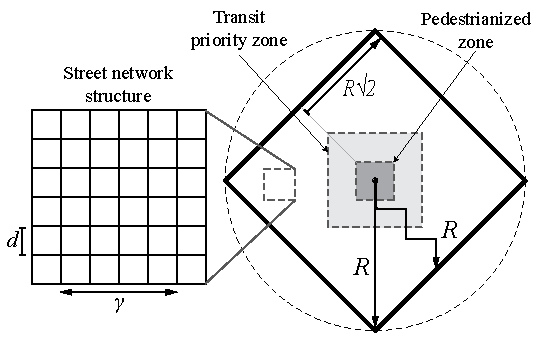
\includegraphics[width=0.5\textwidth]{diagram_pedtransit_grid_city}
     \caption{Rectilinear city with pedestrianized corridor}
     \label{fig:gridcity}
\end{figure}

\noindent The objective is to model the traffic impact on the surrounding street network in order to determine:
\begin{enumerate}[topsep=3pt, itemsep=3pt, partopsep=3pt, parsep=3pt]
    \itshape
    \item what are the optimal pedestrian and transit zone sizes?
    \item what are the impacts on travel time?
    \item what are the resulting shifts in demand?
\end{enumerate}

\section{Demand}
Demand is generated in the city area in units of $\frac{trips}{dist^2}$, and can be simplified into two types: uniform baseline travel across the network, $\lambda_b$, and monocentric travel demand going to and from the center of the city, $\lambda_c$. The pedestrianized zone will cause some trips to be diverted around the perimeter zone. Trips can be categorized into four distinct types (see Figure~\ref{fig:diverted}):

\begin{enumerate}
	\item Unimodal routes unaffected by the pedestrianized zone,
	\item routes taking vehicles around the perimeter of the pedestrianized zone to park nearest the destination and the remaining radial distance is traveled on foot,
	\item routes that would have passed through the center travels around the perimeter of the pedestrianized zone vertically, and
	\item routes that would have passed through the center travels around the perimeter of the pedestrianized zone diagonally.
\end{enumerate}

\begin{figure}[!ht]
     \centering
     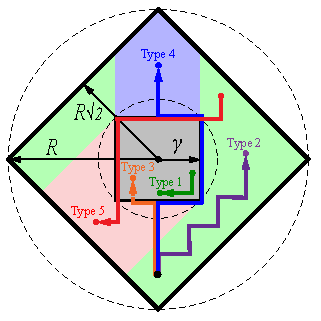
\includegraphics[width=0.3\textwidth]{diagram_diverted_routes}
     \caption{Diverted route types}
     \label{fig:diverted}
\end{figure}

\noindent The flow across the network at a point $r$ distance from the city center is then the summation of this baseline demand and the monocentric demand, calculated as:

\begin{equation}
    q_a(r) = \frac{\lambda_b l}{\delta} + \frac{\lambda_c}{4\delta r} \left(R^2 - r^2 \right)
    \label{eq:flowacross}
\end{equation}

\noindent where $l$ is the average trip link length, $\delta$ is the street density in $\frac{lane \cdot dist}{dist^2}$, calculated as $\delta = \frac{4d}{d^2} = \frac{4}{d}$. The flow around the perimeter road is then calculated as the sum of the flow generated by the four trip types:

\begin{subequations}
\begin{align}
	q_1(\gamma) &= 0 \\
	q_2(\gamma) &= \left[2 \lambda_b \left(R^2 - \gamma^2\right) \times \frac{\gamma^2}{R^2} \times\frac{\gamma}{2}\right] \frac{4d}{8\gamma (R-2)}\\
	q_3(\gamma) &= \left[2 \lambda_b \left(R^2 - \gamma^2\right) \times \frac{\gamma (2R - 3\gamma)}{2R^2} \times  3\gamma\right] \frac{4d}{8\gamma (R-2)}\\
	q_4(\gamma) &= \left[2 \lambda_b \left(R^2 - \gamma^2\right) \times \frac{\gamma (\sqrt{2}R-\gamma)}{R^2} \times  3\gamma\right] \frac{4d}{8\gamma (R-2)}\\
	\notag\text{which can be simplified to:} & \\
	    q_p(\gamma) & = \sum\limits_{i=1}^4 q_i(\gamma) = \frac{\lambda_b d \gamma (6R + 6\sqrt{2}R - 11\gamma)(R^2 - \gamma^2)}{R^2(R-2)}
    \label{eq:perimflow}
\end{align}
\end{subequations}

\noindent The flow across the network at distance $r$ from the center from the function in Equation~\eqref{eq:flowacross} possesses the form shown in Figure~\ref{fig:flowacross}, and flow around the perimeter of the pedestrian zone from the function in Equation~\eqref{eq:perimflow} possesses the form shown in Figure~\ref{fig:perimflow}. As the distance from the city increases, traffic decreases. When traffic near the center exceeds capacity, one might consider simply pedestrianizing the city center out to the point where capacity if first exceeded. However, as the pedestrian zone size increases so does traffic on the perimeter road. 

\begin{figure}[!ht]
     \centering
     \hfill
     \begin{subfigure}[b]{0.45\textwidth}
         \centering
         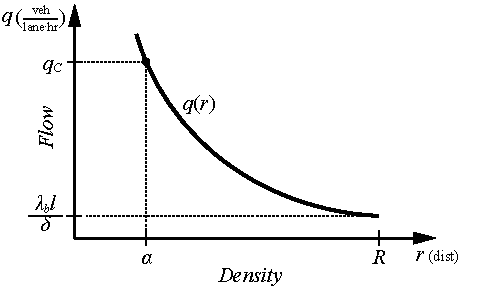
\includegraphics[width=\textwidth]{diagram_flow_across}
         \caption{Trip demand flow at point $r$ distance from center}
         \label{fig:flowacross}
     \end{subfigure}
     \hfill
     \begin{subfigure}[b]{0.45\textwidth}
         \centering
         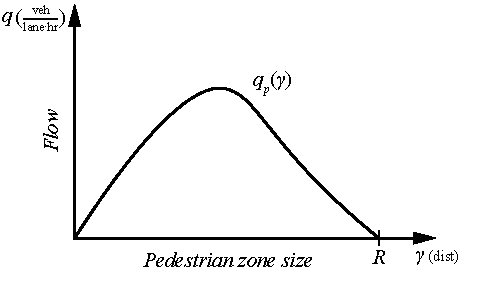
\includegraphics[width=\textwidth]{diagram_flow_perim}
         \caption{Trip demand flow on perimeter of pedestrian zone}
         \label{fig:perimflow}
     \end{subfigure}
     \hfill
     \caption{Macroscopic fundamental diagram and travel time cost function}
\end{figure}

\section{Distance traveled}

Given that only pedestrians, bicycles, and transit may move through the central pedestrian zone, there are three types of trips:
\begin{itemize}
    \item Type 1: Unimodal walking/bicycling trips between two points within the pedestrian zone
    \item Type 2: Bimodal trips when the origin or the destination is located inside the pedestrian zone
    \item Type 3: Unimodal car trips between two points located outside the pedestrian zone
\end{itemize}

\subsection{By foot}
\subsection{By car}
% Also, while moving in the pedestrian area a traveller can only move toward the center or around it 9 by following a circle arc. 10
% A distinction must also be made according to weather a trip is generated by the baseline 11 demand (b) or by the central demand (c). Let ������ ���� be the demand amount and ������ ���� the average walking 12 distance covered in each case �������� where i=1 or 2 and j=c or d. The total distance covered by foot L 13 is then:

% The total distance covered by foot 

% \begin{equation}
%     L = D_{1b}l_{1b} + D_{1c}l_{1c} + D_{2b}l_{2b} + D_{2c}l_{2c}
% \end{equation}

\subsection{By transit}
\subsubsection{In mixed traffic}
\subsubsection{In transit Priority}


\section{Traffic flow}
Traffic flow through the network is characterized by the macroscopic fundamental diagram (see Figure~\ref{fig:mfd}) as a function of density. A travel time function (see Figure~\ref{fig:traveltime}) then depends upon the state of traffic flow through the network as being either ``uncongested'' (solid line) or ``congested'' (dashed line) in Figures~\ref{fig:mfd} and~\ref{fig:traveltime}.

\begin{figure}[!ht]
     \centering
     \hfill
     \begin{subfigure}[b]{0.45\textwidth}
         \centering
         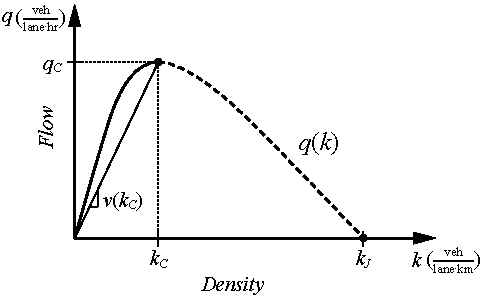
\includegraphics[width=\textwidth]{diagram_mfd}
         \caption{Macroscopic fundamental diagram}
         \label{fig:mfd}
     \end{subfigure}
     \hfill
     \begin{subfigure}[b]{0.45\textwidth}
         \centering
         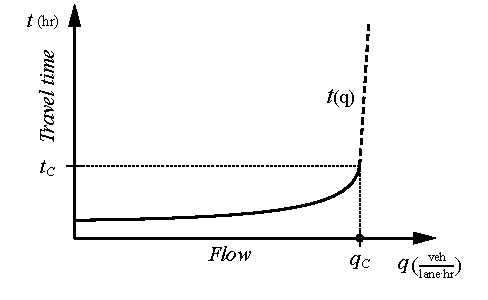
\includegraphics[width=\textwidth]{diagram_traveltime}
        \caption{Travel time cost function}
         \label{fig:traveltime}
     \end{subfigure}
     \hfill
     \caption{Macroscopic fundamental diagram and travel time cost function}
\end{figure}

\noindent A piecewise monotonic cost function for travel time can be defined as:
\begin{subequations}
\begin{align}
    t_D(q) &= l \frac{k(q)}{q} & \text{for}~q < \mu \\
    t_D(q) &= t_c \left(\frac{q}{\mu}\right)  & \text{for}~q \geq \mu
\end{align}
\end{subequations}

\noindent where $t(q)$ is travel time for flow $q$, $k(q)$ is traffic density for flow $q$, $l$ is link length, and $\mu$ is link capacity. Assuming for this case a parabolic function for the uncongested portion of the flow-density relationship, an expression can be written as

\begin{equation}
    q(k) = q_c - (\alpha k - k_c)^2
\end{equation}

\noindent where $k_c$ is the density at capacity, $q_c$ is the flow at capacity, and $\alpha$ is a fitting parameter. In order to determine travel time using density as a function of flow, $k(q)$, it can be solved for using the quadratic formula

\begin{equation}
    k(q) = \frac{k_c - \sqrt{q_c - q}}{\alpha}
    \label{eq:densityparabolic}
\end{equation}


\section{Transit}

Transit travel time is conditional upon whether it operates in a transit priority zone (e.g., dedicated lane or right-of-way) or in mixed-traffic (e.g., city bus). In assuming no other source of delay in a transit priority zone, the travel time of transit is then

\begin{subequations}
\begin{align}
    t_{TP} & = \frac{l}{v_{m}} + \frac{l}{s}t_s  & \text{with transit priority} \\
    t_{TM}(q) & = l\frac{k(q)}{q} + \frac{l}{s}t_s  & \text{without transit priority when}~q \geq \mu\\
    t_{TM}(q) & = t_c \left(\frac{q}{\mu}\right) + \frac{l}{s}t_s & \text{without transit priority when}~q \geq \mu
\end{align}
\end{subequations}

\noindent where $v_m$ is the maximum cruising speed of transit unimpeded by traffic, $s$ is stop spacing, and $t_s$ is stop time. The stop time is essentially the lost time inclusive of acceleration, deceleration and dwell time.

The travel time of transit in mixed-traffic will then always be higher than driving an automobile, eventually converging as traffic conditions reach jam flow. Transit priority provides a constant travel time which will be initially slower than driving in uncongested traffic conditions, but will eventually reach a traffic flow point $q^*_T$, where the travel time of transit with priority exceeds driving (see Figure~\ref{fig:transittraveltime}).

\begin{figure}[!ht]
     \centering
     \hfill
     \begin{subfigure}[b]{0.45\textwidth}
         \centering
         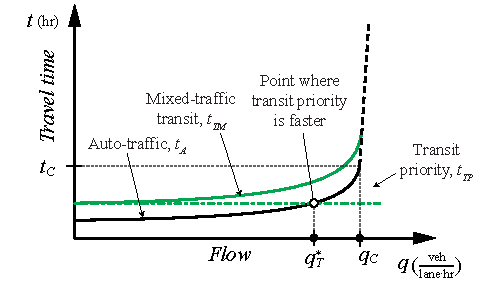
\includegraphics[width=\textwidth]{diagram_transit_traveltime}
        \caption{Transit travel time}
         \label{fig:transittraveltime}
     \end{subfigure}
     \hfill
     \begin{subfigure}[b]{0.45\textwidth}
         \centering
         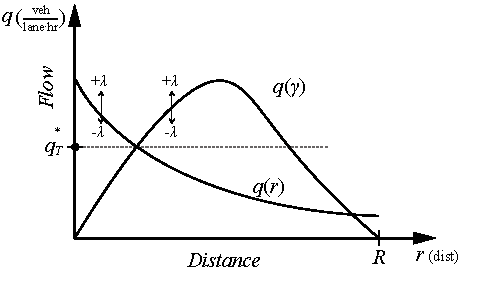
\includegraphics[width=\textwidth]{diagram_flow_combo}
         \caption{Optimal pedestrian and transit priority zone size}
         \label{fig:flowcombo}
     \end{subfigure}
     \hfill
     \caption{Transit travel time and optimal zone sizing}
\end{figure}

The critical transit priority traffic flow point $q^*_T$, if found where transit travel time $t_{TP}$ intersects driving travel time $t_D{q}$. Assuming the parabolic traffic flow function in Equation~\eqref{eq:densityparabolic}, the critical transit priority traffic flow point is:

\begin{equation}
    q^*_T = \alpha^2 \left( \frac{1}{v_m} - \frac{t_s}{s} \right)^2 - k_c^2 + q_c
\end{equation}

\noindent $q^*_T$ could then be used in combination with network flow at distance $r$ in Equation~\eqref{eq:flowacross} to determine the optimal transit priority zone, $\tau^*$. The solution to this is quadratic, but assuming a non-negative value for the optimal transit zone size, it can be solved for analytically:

\begin{equation}
    \tau^* = \frac{2\left(q_{t}\delta-\lambda_{b}R\right)-\sqrt{4\left(q_{t}\delta-\lambda_{b}R\right)^{2}+\lambda_{c}^{2}R^{2}}}{\lambda_{c}}
\end{equation}

Determining an optimal pedestrian zone size is slightly more complex. An appropriate pedestrian zone size can exist anywhere in the range $q_a(\gamma) < q_c > q_p(\gamma)$ where the pedestrian zone is (see Figure~\ref{fig:flowcombo}):

\begin{enumerate}[label=(\alph*)]
    \item large enough to prevent traffic flow across the network from exceeding capacity $q_a(\gamma) < q_c$, and 
    \item small enough to prevent perimeter traffic flow from exceeding capacity $q_p(\gamma) < q_c$. 
\end{enumerate}

The intersection point of the two functions may be used as an optimal compromise, ensuring both conditions are satisfied with the least possible traffic flow. However, setting $q_a = q_p$ to find the intersection point results in a quintic function (polynomial to the $5^{th}$ power):

\begin{equation}
f(\gamma) =  \frac{11}{R^2} \gamma^5 - \frac{6(1+\sqrt{2})}{R}\gamma^4 - 11\gamma^3 + \frac{24\delta\lambda_b d R(1+\sqrt{2}) + \lambda_{c}(R-2)}{4\delta\lambda_{b}d}\gamma^{2} - \frac{R(R-2)}{\delta d}\gamma - \frac{\lambda_{c}(R-2)R^{2}}{4\delta\lambda_{b}d}
\end{equation}

\noindent yielding multiple points where the function is equal to zero (see Figure~\ref{fig:optimalped}) and cannot be easily solved analytically.

\begin{figure}[!ht]
     \centering
     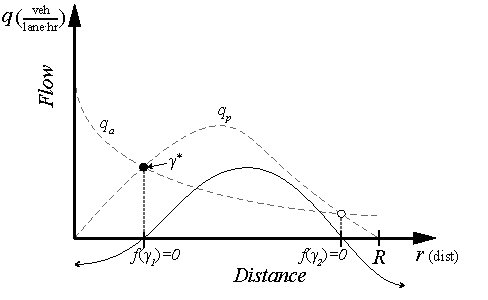
\includegraphics[width=0.6\textwidth]{diagram_optimalped}
     \caption{Quintic function for optimal pedestrian zone size, $f(\gamma)$}
     \label{fig:optimalped}
\end{figure}

Given that the pedestrian zone size must exist between $0 \leq \gamma \leq R$ an optimal pedestrian zone dimension $\gamma^*$, can be found numerically. Since two intersection points between $q_a$ and $q_p$ exist, the minimum of the two provides the desired optimal $\gamma^*$:

\begin{align}\small
\gamma^* &\Leftarrow \text{min} \left[ f(\gamma_1) = 0, f(\gamma_2) = 0 \right]\\
\text{s.t.} & ~ 0 \leq \gamma \leq R 
\end{align}


\section{Mode choice}
Assuming unlimited transit capacity relative to driving and that transit priority is unaffected by congestion, a transit system with transit priority in this model effectively serves as a pressure release for demand. As congestion increases with driving trips, transit becomes more appealing, thus drawing trips away from driving. Conversely, a reduction in congestion would attract trips towards driving as the driving travel time has improved. Assuming transit provides a reasonable and reliable alternative to driving, some demand equilibrium exists where the travel time cost of driving matches transit.

The mode choice can be modeled as the probability of choosing to drive $P_D$ or transit $P_T$, using a simple two-alternative logit model with (dis-)utility as the choice travel cost:

\begin{subequations}
    \label{eq:choiceprob}
    \begin{align}
        P_D & = \frac{1}{1+e^{-\beta (t_D-t_T)}}\\
        P_T & = 1 - P_D
    \end{align}
\end{subequations}

\noindent where $t_D$ and $t_T$ are the travel times associated with automobile and transit, respectively; and $\beta$ is the a estimated scaling parameter. The probability in Equation~\eqref{eq:choiceprob} can be used to find the proportion of trips made by driving.


\section{...}

A two-alternative logit can be simplified to require only the cost difference between the two choices, not the full value, thus logit only requires a travel time differential $\Delta t = t_D - t_T$:

\begin{equation}
    \Delta t(q) = l \frac{k(q)}{q} - \left[
    \frac{\tau}{R} \left( \frac{l}{v_T} + \frac{l}{s}t_s \right) + \frac{R-\tau}{R} \left( l\frac{k(q)}{q} + \frac{l}{s}t_s \right) \right]
\end{equation}

\noindent Since $q^*_T$ is a global constant regardless of demand, we can get $\tau$ by setting $q_a(\tau)=q^*_T$. But $q_a$ depends on demand, which depends on probability, which depends on travel time.

\begin{align}
    q_a(\tau, \Delta t(q)) & = P_D(\Delta t(q)) \times \left[ \frac{\lambda_b l}{\delta} + \frac{\lambda_c}{4\delta} \left( \frac{R^2}{\tau} - \tau \right) \right] \\
    q_a(\tau, \Delta t(q)) & = q^*_T
\end{align}

\noindent Now there is some sort of dynamic equilibrium with flow and demand where travel time depends on flow and flow depends on travel time. 

The pedestrian zone size somewhat less critical since it can exist in a range. However, lets set boundary as the perimeter flow.

\begin{equation}
        q_p(\gamma, \Delta t(q)) = P_D(\Delta t(q)) \times \frac{\lambda_b d \gamma (R^2 - \gamma^2) (3R + 3\sqrt{2}R - 7\gamma)}{R^2(R-2)} < q_c
\end{equation}


\end{document}
